\chapter{State of the art}

% INTRODUCTION %

In this chapter we analyze the current state of \<Level Design> and of its common practices, both in academic and in professional environments, with attention to the genre of \<First Person Shooters> (or \<FPS>).

\par

We then talk about \<Procedural Content Generation> (or \<PCG>), focusing on how it allows to enrich and ease the design process.

\par

After that, we give an overview of the First Person Shooter genre, analyzing its features, history and evolution, devoting special attention to the games that mostly contributed to the definition of this genre.

\par

Finally, we analyze how Graph Theory has been in used in Video Games during the years.

% LEVEL DESIGN %

\section{Level Design Theory}

\<Level Design> is a game development discipline focused on the creation of video game levels.

\par

Today, the level designer is a well-defined and fundamental figure in the development of a game, but it was not always so. In the early days of the video game industry, it was a widespread practice to assign the development of levels to members of the team with other roles, usually programmers. Apart from the limited number of team members and the low budget, this was because there were no tools such as \<level editors>\footnote{\label{levelEditorFootnote}A level editor is a software used to design levels, maps and virtual worlds for a video game.}, that allowed the level designer to work on a level without being involved with code.

\par

The level designer has a really significant role in the development of a good game, since he is responsible for the creation of the world and for how the player interacts with it. The level designer takes an idea and makes it tangible. Despite the importance of this process, after all this years it has not been established a common ground or a set of standards and level design is still considered as a form of art, based on heuristics, observation, previous solutions and personal sensibility.

\par

In addition to gameplay, the game designer must consider the visual appearance of the level and the technological limitations of the \<game engine>\footnote{\label{gameEngineFootnote}A game engine is a software framework designed for the creation and development of video games.}, combining all this elements in a harmonic way.

\par

One of the core components of level design is the \[``level flow'']. For single player games it translates into the series of actions and movements that the player needs to perform to complete a level. A proficient level design practice is to guide the player in a transparent way, by directing his attention towards the path he needs to follow. This can be achieved in diverse ways. Power ups and items can be used as breadcrumbs to suggest the right direction in a one-way fashion, since they disappear once picked up. Lighting, illumination and distinctly colored objects are another common approach to this problem. A brilliant example of this is \<Mirror's Edge>\footnote{Digital Illusions CE, 2008.}, which uses a really clear color code, with red interactive objects in an otherwise white world, to guide the player through its fast-paced levels. There are also even more inventive solutions, like the dynamic flock of birds in \<Half Life 2>\footnote{Valve, 2004.}, used to catch the player attention or to warn him of incoming dangers\cite{GuidingThePlayersEye}. Finally, sounds and architectures are other elements that can be used to guide the player. In the academic environment, a lot of researchers have analyzed the effectiveness of this kind of solutions: Alotto\cite{HowLevelDesignersAffect} considers how architecture influences the decisions of the player, whereas Hoeg\cite{TheInvisibleHand} also considers the effect of sounds, objects and illumination, with the last being the focus of Brownmiller's\cite{InGameLigthing} work.

\par

In multiplayer games the level flow is defined by how the players interact with each other and with the environment. Because of this, the control of the level designer is less direct and is exercised almost exclusively by modeling the map. Considering FPS, the level flow changes depending on how much an area is attractive for a player. The more an area is easy to navigate or offers tactical advantage, such as covers, resources or high ground, the more players will be comfortable moving in it. This doesn't mean that all areas need to be designed like this, since zones with a ``bad'' flow but an attractive reward, such as a powerful weapon, force the player to evaluate risks and benefits, making the gameplay more engaging. The conformation of the map and the positioning of interesting resources are used to obtain what Güttler et al.\cite{Guttler:2003:SPL:963900.963915} define as ``points of collisions'', i.e. zones of the map were the majority of the fights are bound to happen. 

\par

Moving back to academic research, Güttler et al. have also noticed how aesthetic design loses importance in a multiplayer context. Other researches are instead focused on finding \[patterns] in the design of multiplayer maps: Larsen\cite{LevelDesignPatterns} analyzes three really different multiplayer games, \<Unreal Tournament 2004>\footnote{Epic Games, 2004.}, \<Day of Defeat: Source>\footnote{Valve, 2005.} and \<Battlefield 1942>\footnote{DICE, 2002.}, identifying shared patterns and measuring their effect on gameplay, suggesting some guidelines on how to use them, whereas Hullet and Whitehead identify some patterns for single player games\cite{Hullett:2010:DPF:1822348.1822359}, many of whom are compatible with a multiplayer setting, with Hullett also proving cause-effect relationships for some of this patterns by confronting hypothesized results with the ones observed on a sample of real players\cite{TheScienceOfLevelDesign}. Despite these experimental results contributing to a formalization of level design, we are still far from a structured scientific approach to the subject.

% PROCEDURAL CONTENT GENERATION %

\section{Procedural Content Generation}

\<Procedural Content Generation> refers to a family of algorithms used to create data and content in an automatic fashion. In game development it is commonly used to generate weapons, objects, maps and levels, but it is also employed for producing textures, models, animations, music and dialogues.

\par

The first popular game to use this technique was \<Rogue>\footnote{Michael Toy, Glenn Wichman, 1980.}, an ASCII dungeon exploration game released in 1980, where the rooms, hallways, monsters, and treasures the player was going to find were generated in a pseudo-random fashion at each playthrough. Besides providing a huge replay value to a game, PCG allowed to overcome the strict memory limitations of the early computers. Many games used pseudo-random generators with predefined \<seed values> to create very large game worlds that appeared to be premade. For instance, the space exploration and trading game \<Elite>\footnote{David Braben, Ian Bell, 1984.} contained only eight galaxies, each one with 256 solar systems, of the possible 282 trillion the code was able to generate, since the publisher was afraid that such an high number could cause disbelief in the players. Another example is the open world action role-playing game \<The Elder Scrolls II: Daggerfall>\footnote{Bethesda Softworks, 1996.}, which game world has the same size of Great Britain. 

\par

As computer hardware advanced and the size of the memory increased, procedural generation of game worlds was generally put aside, since it could not compete with the level of detail that hand-crafted worlds were able to achieve.

\par

However, in the last years, with the players' expectations and the production value of video games constantly increasing, procedural generation made a comeback as a way to automate the development process and reduce costs. Many \<middleware> tools, such as \<SpeedTree>\footnote{IDV, Inc.} and \<World Machine>\footnote{World Machine Software, LLC.}, are used to produce various kind of content, like terrain and natural or artificial environments.

\par

Many modern \<AAA>\footnote{Video games produced and distributed by a major publisher, typically having high development and marketing budgets.} games use procedural generation: in \<Borderlands>\footnote{Gearbox Software, 2009.} a procedural algorithm is responsible for the generation of guns and other pieces of equipment, with over a million unique combinations; in \<Left 4 Dead>\footnote{Valve, 2008.} an artificial intelligence is used to constantly make the players feel under threat, by dynamically changing the music, spawning waves of enemies and changing the accessible paths of the level; in \<Spore>\footnote{Maxis, 2008.} \<procedural animation> is employed to determine how the creatures created by the player move.

\par

Nowadays, PCG is widely used by \<independent> developers, that, lacking the high budgets of AAA games, try to obtain engaging and unusual gameplay using unconventional means. The most famous example is \<Minecraft>\footnote{\label{ }Mojang, 2011.}, a sandbox survival game which worlds, composed exclusively by cubes, are generated automatically. Currently, the most extreme form of procedural generation is the one found in \<No Man's Sky>\footnote{Hello Games, 2016.}, a space exploration game where space stations, star-ships, planets, trees, resources, buildings, animals, weapons and even missions are generated procedurally. Following in the footstep of their forefather, many roguelike games still use PCG, like \<The Binding of Isaac>\footnote{Edmund McMillen, 2011.}.

\par

All the algorithms used by these games and middleware are designed to be as fast as possible, since they need to generate the content in real time. In the last years researchers have nevertheless tried to explore new paradigms, creating more complex procedural generation techniques, that allow for a tighter control on the output. Being one of the problems of PCG the lack of an assured minimum quality on the produced content, the academic environment has focused not only on more advanced generation algorithms, but also on techniques to evaluate the output itself in an \<automatic> fashion. In this field, Togelius et al.\cite{10.1007/978-3-642-12239-2_15} defined \<Search-Based Procedural Content Generation>, a particular kind of \<Generate-And-Test>\footnote{Algorithms with both a generation and an evaluation component, that depending on some criterion, decide to keep the current result or to generate a new one.} algorithm, where the generated content, instead of being just accepted or discarded, is evaluated assigning a \<suitability score> obtained from a \<fitness function>, used to select the best candidates for the next iterations.

% PROCEDURAL CONTENT GENERATION IN FPSES %

\section{Procedural Content Generation for FPS maps}

We have really few examples of commercial FPS that use PCG to generate their maps: with the exception of \<Soldier of Fortune II: Double Helix>\footnote{ Raven Software, 2002.}, that employs these techniques to generate whole missions, the few other cases we have are all roguelikes with a FPS gameplay, like \<STRAFE>\footnote{Pixel Titans, 2017.}.

\par

Despite the total lack of FPS using procedural generation to obtain multiplayer maps, researchers have proved that search-based procedural content generation can be an useful tool in this field. In a seminal work, Cardamone et al.\cite{Cardamone:2011:EIM:2008402.2008411} tried to understand which kind of \<deathmatch>\footnote{A widely used multiplayer game mode where the goal of each player is to kill as many other players as possible until a certain end condition is reached, commonly being a kill limit or a time limit.} maps created the most enjoyable gameplay possible. To achieve this, the authors generated maps for \<Cube 2: Sauerbraten>\footnote{Wouter van Oortmerssen, 2004} by maximizing a fitness function computed on \<fight time> data collected from \<simulations>\footnote{In the field of search-based procedural generation, fitness function based on simulation are computed on the data collected from a match between artificial agents in the map at issue. They differ from \<direct> and \<interactive> functions, that evaluate, respectively, the generated content and the interaction with a real player.}, with the fight time being the time between the start of a fight and the death of one of the two contenders. The choice of this fitness function is based on the consideration that a long fight is correlated with the presence of interesting features in the map, such as escape or flanking routes, hideouts and well positioned resources. 

\par

Stucchi et al.\cite{EvoluzioneMappeBilanciate}, yet remaining in the same field, attempted a completely different use of procedural generation, by producing balanced maps for player with different weapons or different levels of skill. For doing so, they generated procedural maps via evolutionary algorithms, evaluating them with a fitness function based on simulation that computes the entropy of kills. Starting from a situation where one of the two players has a significant advantage, they proved that changes in the map structure allow to achieve a significant balance increase.

\par

Arnaboldi\cite{SviluppoDiUnFramework} combined these two approaches, creating a framework that automatically produces maps using a genetic process like the one of Cardamone. In Arnaboldi's work, however, the fitness function is way more complex, since it considers a high number of gameplay metrics, and the AI of the employed \<bots>\footnote{The artificial players of a video game.} is closer to the one of a human player, thanks to a series of adjustments made to the stock \<Cube 2> one. These improvements significantly increase the flexibility of the framework and the overall quality of the output, allowing to identify and analyze some recurring patterns and their relationship with the statistics gathered during the simulations. 

\par

Ølsted et al.\cite{DesignerJob} moved the focus of their research from deathmacth to squad game modes with specific objectives, sustaining not only that the maps generated by Cardamone et al. are not suitable for this kind of gameplay, but also that they do not conform to what they define as \<The Good Engagement> (or \<TGE>) rules, i.e. a set of rules that a FPS should satisfy to support and encourage interesting player choices, from which an engaging gameplay should emerge naturally. By analyzing the \<Search \& Destroy>\footnote{A multiplayer game mode where players, divided in two teams, have to eliminate the enemy team or detonate a bomb in their base.} mode of games like \<Counter Strike>\footnote{Valve Software, 2000} and \<Call of Duty>\footnote{Infinity Ward, 2003}, they defined a process to generate suitable maps: starting from a grid, some nodes are selected and connected among them, the result is then optimized to satisfy the TGE rules and finally rooms, resources, objects and spawn points are added, as can be seen in figure \ref{fig:olstedGenerativeProcess}. Opting for an \<interactive> approach, the fitness function used to guide the evolution of these maps is computed on the binary appreciation feedback expressed by real users, since the authors consider bot behavior too different form the one of real users.

\begin{figure}
  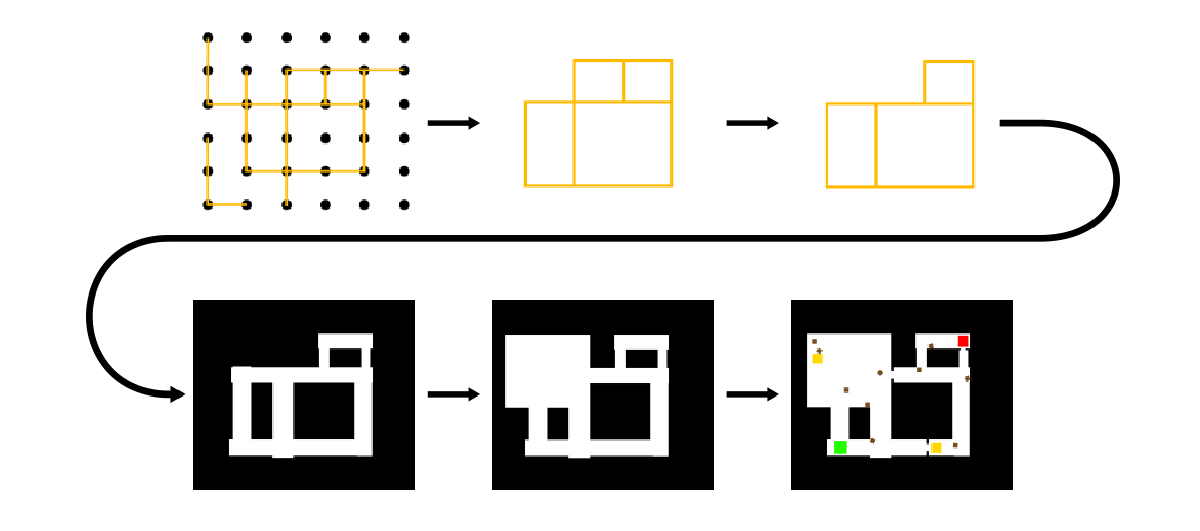
\includegraphics[width=\linewidth]{olstedGenerativeProcess}
  \caption{Visual representation of Ølsted et al.\cite{DesignerJob} generative process.}
  \label{fig:olstedGenerativeProcess}
\end{figure}

A completely different approach from the ones listed above is the one of Anand and Wong\cite{10.1007/978-3-662-45212-7_19}, who employed search-based procedural generation to create \<online>, automatically and rapidly multiplayer maps for the \<Capture and Hold>\footnote{A multiplayer game mode where players, divided in two teams, fight for the control of some strategic areas. The score of each team increases over time proportionally to the number of controlled points until one of the two teams reaches a given limit, winning the game.} game mode, without compromising the quality of the final output. To achieve this, they employ a genetic approach, which fitness function is evaluated directly on the topology of the map, considering four different factors: the connectivity between regions, the number of points of collision, the balancing in the positioning of control points and spawn points. With no need to simulate matches, this process can be completed in a matter of seconds. The algorithm starts by generating three maps, that are then evolved by mutation. To obtain the initial maps, Anand and Wong populate a grid with random tiles, they clean it of undesired artifacts and they identify regions within it, that are then populated with strategic points, resources, spawn points and covers. Despite its good results, this approach heavily relies on the validity of the selected topological metrics and, as we have seen, it is still not clear which the good elements of a level are.

\par

Finally, Cachia et al.\cite{MultiLevelEvolution} extended search-based procedural generation to multi-level maps, generating the ground floor with one of the methods defined by Cardamone and employing a random digger for the first floor. The final result can be seen in figure \ref{fig:multiLevelEvolution1}. Their algorithm also positions spawn points and resources through a topological fitness function, which entails the same problems described for Anand and Wong's approach.

\begin{figure}
  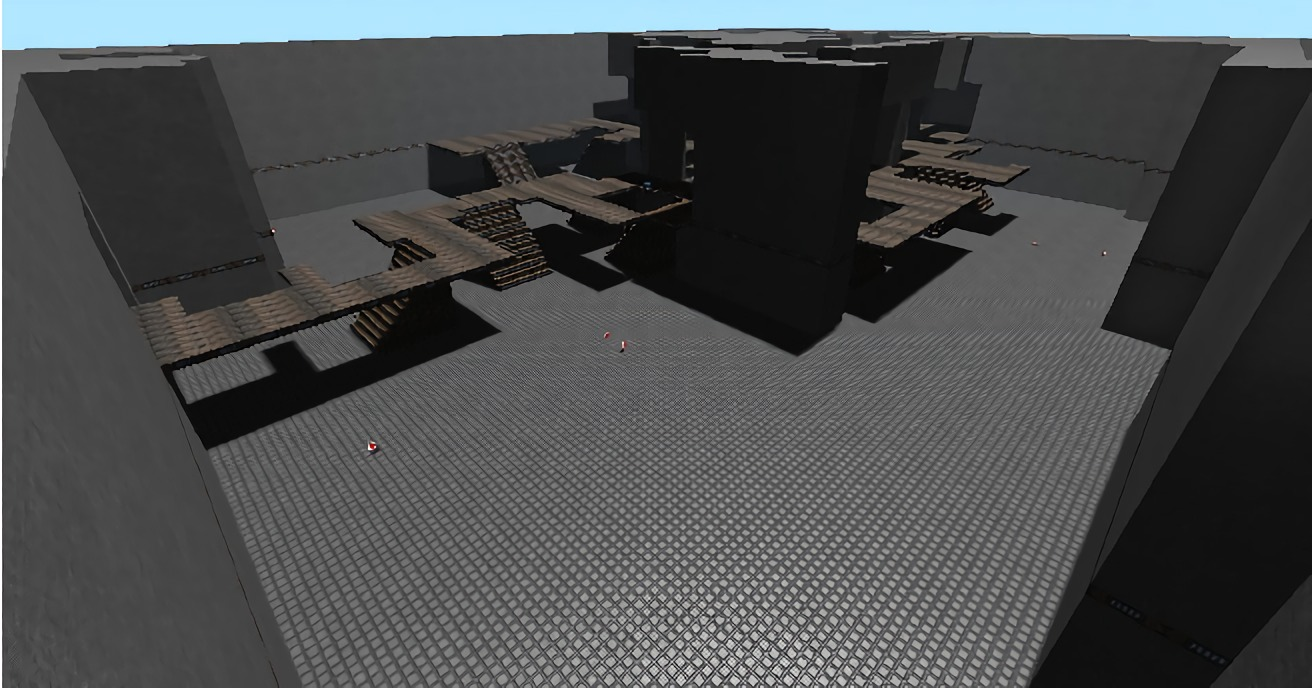
\includegraphics[width=\linewidth]{multiLevelEvolution}
  \caption{One of the maps evolved by Cachia's et al.\cite{MultiLevelEvolution} algorithm.}
  \label{fig:multiLevelEvolution1}
\end{figure}

% FPS DESIGN %

\section{History of Level Design in FPS}

\<First Person Shooter> are a video game genre which main features are the first-person player perspective and a weapon-based combat gameplay. During the years this genre has been consonantly evolving, as new elements started to emerge from the very aggressive and fast-paced gameplay of the first games of this kind, like \<Doom>\footnote{ID Software, 1993.}. Games like \<Half-Life>\footnote{Valve Software, 1998.} highlighted the importance of the story and of the setting, games like \<Deus Ex>\footnote{Ion Storm, 2000.} introduced role-play and stealth mechanics and games like \<Quake III: Arena>\footnote{id Software, 1999.} and \<Unreal Tournament>\footnote{Epic Games, 1999.} moved the focus from single player to multiplayer. Finally, Modern Military Shooters introduced a slower and more realistic gameplay and radically changed the setting from fictional conflicts to contemporary ones.

\subsection{Level Design evolution in FPS}

The evolution of the mechanics of this genre was supported by a constant refinement of level design and of the used tools.

\paragraph{Before 1992: The first FPS}

\mbox{}\\

{\setlength{\parindent}{0cm}
The origin of the FPS genre goes back to the beginning of video games themselves. In 1973, Steve Colley developed \<Maze War>, a simple black-and-white multiplayer game set in a tile-based maze, where players would search for other players' avatars, killing them to earn points. Around the same time, Jim Bowery created \<Spasim>, a simple first-person space flight simulator. Both games were never released, instead, we must wait the beginning of the 80's to see the first products available to the public. Heavily inspired by Colley and Bowerey's work, these games had almost no level design, but during the years they started to become a little more complex, with tangled sci-fi structures taking over mazes. 
}

\paragraph{1992: Wolfenstein 3D defines a new genre}

\mbox{}\\

{\setlength{\parindent}{0cm}
When \<Wolfenstein 3D>\footnote{id Software, 1992.} was released in 1992, it changed the genre forever, thanks to its fast gameplay and its light game engine, that allowed to target an audience as wide as possible. Wolfenstein 3D took up the exploitative approach of the period, with its levels full of items, weapons and secret rooms. The level design was still simple, because the technical limitations of the engine and of its \<tile-based>\footnote{The map consists in a grid composed by squared cells, or \<tiles>, of equal size.} \<top-down>\footnote{In \<top-down> games and editors, the game world is seen from above.} level editor allowed to create only flat levels, with no real floor or ceiling and walls always placed at a right angle. 
}

\paragraph{1993 - 1995: Doom and its legacy}

\mbox{}\\

{\setlength{\parindent}{0cm}
A year later, id Software released \<Doom>, a milestone in the history of the genre. The game engine of Doom was capable of many innovations: sections with floor and ceiling with variable height, elevators, non-orthogonal walls, interactive elements, lightning, even dynamic, textures for horizontal surfaces and even a simple \<skybox>\footnote{A method of creating backgrounds that represent scenery in the distance, making the game world look bigger than it really is.}, all of this without losing the speed that characterized Wolfenstein. The developers took advantage as much as possible of the capabilities of the engine, achieving a level design way more complex than what had been seen before. In addition, Doom was designed to be easily modifiable by the users and featured cooperative and competitive multiplayer, via LAN or dial-in connections, that rapidly gathered a massive user base.
}

\par

The impact of Doom on the genre was so strong that in the following years the market was flooded with its clones. All these games, as well as Doom, had still some technical limits, in their engines, that were not completely 3D, in their level editors, that were still top-down and did not allow for the design of more complex levels, and in their gameplay, that still faced limited movements.

\paragraph{1996 - 2000: A constant evolution}

\mbox{}\\

{\setlength{\parindent}{0cm}
In the next years, many games continued what Doom started, bringing constant improvements to the genre. \<Duke Nukem 3D>\footnote{3D Realms, 1996.} set aside the sci-fi settings of its predecessors, switching to real locations, inspired by the ones of Los Angeles. This was possible thanks to its \<2.5D>\footnote{A \<2.5D> engine renders a world with a two dimensional geometry in a way that looks three-dimensional. An additional height component can be introduced, allowing to render different ceiling and floor height. This rendering technique limits the movements of the camera only to the horizontal plane. Doom and many similar games employed this technology.} engine \<Build>\footnote{Developed by Ken Silverman in 1995.}, that provided a \<What You See Is What You Get>\footnote{In computer science, \<What You See Is What You Get > denotes a particular kind of editors where there is no difference form what you see during editing and the final output.} level editor. Furthermore, Build allowed to apply \<scripts> to certain elements of the map, resulting in a more interactive environment.
}

\par

Released in 1996, \<Quake>\footnote{id Software, 1996.} was one of the first and most successful FPS with a real 3D engine, that allowed an incredible jump forward in terms of realism, level design and interactivity. Quake had also a rich multiplayer, with a lot of maps, game modes and special features, like clans and modding. Two years later, \<Unreal>\footnote{Epic Games, 1998.} brought a new improvement in terms of realism and level design, thanks to its engine capable of displaying huge outdoors settings.

\par

In those years many new sub-genres started to spawn, obtained by emphasizing certain features of the previous games or by borrowing mechanics from other genres. \<Quake III Arena>\footnote{id Software, 1999.} and \<Unreal Tournament>\footnote{Epic Games, 1999.} were some of the first and most successful multiplayer games ever released, that required a new approach to level design, completely focused on the creation of competitive maps. Games like \<Deus Ex> introduced tactical and RPG elements, with the possibility of reaching an objective in multiple ways, thanks to a level design that exalted the freedom left to player. Finally, \<Half-Life> changed forever the approach of this genre to storytelling and to level design: the game puts great emphasis on the story, that is narrated from the eyes of the player, without cut-scenes, and introduces the possibility of moving freely between areas, with no interruption. The game also set new standards with its challenging enemy AI, capable of taking advantage of the terrain and coordinating flanking maneuvers. 

\paragraph{2001: The rise of console shooters}

\mbox{}\\

{\setlength{\parindent}{0cm}
In 2001, \<Halo: Combat Evolved>\footnote{Bungie, 2001.} revolutionized the genre, introducing some of the mechanics on which modern FPS are based, as the limited amount of weapons that the player can carry and the regeneration of health over time. This slower and more strategic approach to gameplay matched perfectly with consoles and their twin-stick-controllers, that were not suitable for the extremely fast paced action of the past. Over time, this new approach to gameplay overshadowed almost completely all the others, thanks to the diffusion of consoles and to the increase of production costs, that made PC exclusives economically disadvantageous. From the standpoint of level design, this change required to increase the complexity of the levels and the addition of strategically placed covers.
}

\paragraph{Today: A time of stagnation}

\mbox{}\\

{\setlength{\parindent}{0cm}
Starting from its origins, level design undergone a radical evolution, but in the last years it has shown no significant improvements. This could be due to the considerable risk associated with modern projects or to the lack of suitable instruments.
}

% GRAPH THEORY %

\section{Graph Theory in video games}

\<Graph Theory> has always been used in video games, usually as a useful tool to perform \<pathfinding> for artificial agents. These techniques revolve around the creation of a \<navigation mesh>, i.e. a representation of the walkable areas of a level using non-overlapping polygons obtained by removing the shapes of obstacles from the considered surface. The result is then used to generate a graph, selecting as nodes the vertices or the centers or the centers of edges of the obtained polygons, depending on the kind of movement that must be achieved. This graph can be pre-generated or computed at run-time, if the technique is applied to dynamic environments. Finally, an algorithm like \<A*> is employed to find the shortest path between two points. This process can be seen in figure \ref{fig:pathfinding}

\par

Graphs are also used in procedural generation, as an effective tool to model landmasses and roads.

\begin{figure}
  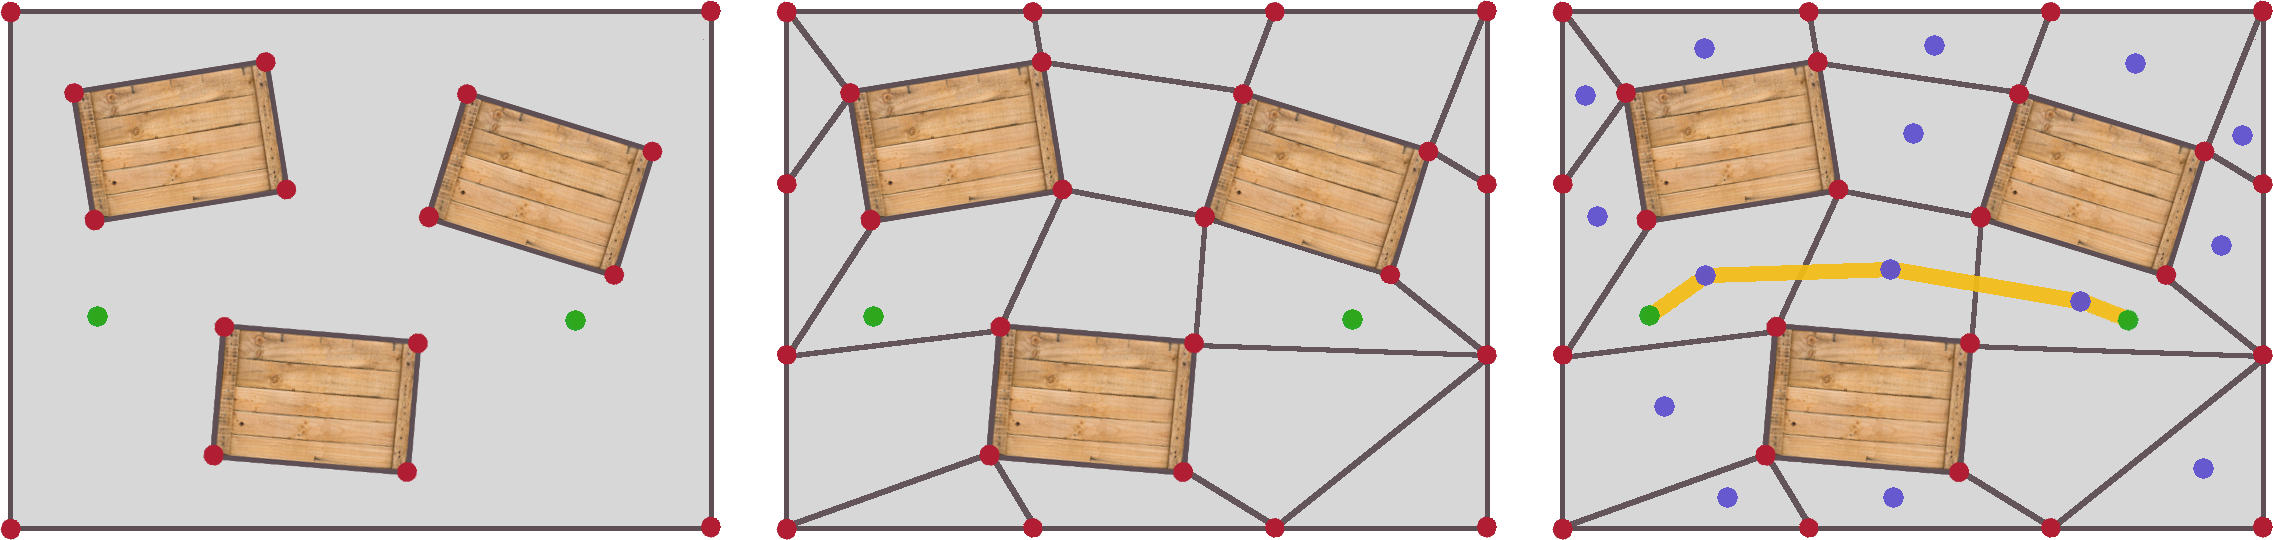
\includegraphics[width=\linewidth]{pathfinding}
  \caption{A common pathfinding process.}
  \label{fig:pathfinding}
\end{figure}

% SUMMARY %

\section{Summary}

In this chapter we analyzed the current state of level design for First Person Shooters and how this field has been explored in academic research. We then introduced Procedural Content Generation and we observed how some studies have proved that it is a suitable method to produce maps for FPS games. We also took a brief look at the history of First Person Shooters, analyzing how level design evolved over time. Finally, we depicted some of the most common uses of Graph Theory in video games. 